% 97-50(97쪽) — 직육면체 ABCD-EFGH 와 그 안의 삼각형 AFC(원문 「오른쪽 그림」). 스캔 화질이 낮아 TikZ 로 다시 그림.
% 보이는 모서리는 실선, 숨은 모서리(DH·HG·HE)는 점선. 라벨은 원문 것만: 꼭짓점 여덟 개와 $2\sqrt{2}$(AD·BC)·$1$(BF).
% 삼각형 AFC 의 넓이(답)가 읽히지 않게 다른 길이는 적지 않는다.
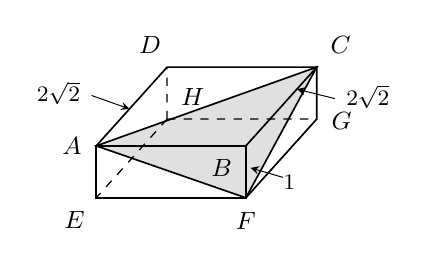
\begin{tikzpicture}[line width=0.6pt, x=1cm, y=1cm, >=stealth]
  \coordinate (A) at (0,0.66);
  \coordinate (B) at (1.90,0.66);
  \coordinate (E) at (0,0);
  \coordinate (F) at (1.90,0);
  \coordinate (D) at (0.90,1.66);
  \coordinate (C) at (2.80,1.66);
  \coordinate (H) at (0.90,1.00);
  \coordinate (G) at (2.80,1.00);
  \fill[black!12] (A) -- (F) -- (C) -- cycle;
  \draw[dashed, line width=0.45pt] (H) -- (D) (H) -- (G) (H) -- (E);
  \draw (A) -- (B) -- (F) -- (E) -- cycle;
  \draw (A) -- (D) -- (C) -- (B);
  \draw (C) -- (G) -- (F);
  \draw (A) -- (F) -- (C) -- cycle;
  % 길이 표시
  \node[font=\footnotesize] at (-0.48,1.33) {$2\sqrt{2}$};
  \draw[->, line width=0.35pt] (-0.06,1.30) -- (0.42,1.13);
  \node[font=\footnotesize] at (3.45,1.28) {$2\sqrt{2}$};
  \draw[->, line width=0.35pt] (3.03,1.26) -- (2.55,1.38);
  \node[font=\footnotesize] at (2.45,0.20) {$1$};
  \draw[->, line width=0.35pt] (2.37,0.26) -- (1.96,0.38);
  \node[font=\small, anchor=south east] at (0.95,1.70) {$\pt{D}$};
  \node[font=\small, anchor=south west] at (2.85,1.70) {$\pt{C}$};
  \node[font=\small, anchor=east] at (-0.06,0.66) {$\pt{A}$};
  \node[font=\small, anchor=north east] at (1.85,0.62) {$\pt{B}$};
  \node[font=\small, anchor=south west] at (0.95,1.04) {$\pt{H}$};
  \node[font=\small, anchor=west] at (2.86,0.98) {$\pt{G}$};
  \node[font=\small, anchor=north east] at (-0.02,-0.04) {$\pt{E}$};
  \node[font=\small, anchor=north] at (1.90,-0.06) {$\pt{F}$};
\end{tikzpicture}
